\documentclass[12pt]{article}
\usepackage[utf8]{inputenc}
\usepackage{graphicx} % Allows you to insert figures
\usepackage{amsmath} % Allows you to do equations
\usepackage{fancyhdr} % Formats the header
\usepackage{geometry} % Formats the paper size, orientation, and margins
\usepackage[style=authoryear-ibid,backend=biber]{biblatex} % Allows you to do citations - does Harvard style and compatible with Zotero

% PARA IMAGNES E SUBIMAGENS
\usepackage{graphicx}
\usepackage{subcaption}
\usepackage{mwe}

\usepackage[section]{placeins}
\usepackage{hyperref}
\usepackage{listings}

\usepackage{amsmath}

\addbibresource{Example.bib} % Tells LaTeX where the citations are coming from. This is imported from Zotero
\usepackage[english]{babel}
\usepackage{csquotes}
\renewcommand*{\nameyeardelim}{\addcomma\space} % Adds comma in in-text citations
\linespread{1.25} % About 1.5 spacing in Word
\setlength{\parindent}{0pt} % No paragraph indents
\setlength{\parskip}{1em} % Paragraphs separated by one line
\renewcommand{\headrulewidth}{0pt} % Removes line in header
\geometry{legalpaper, portrait, margin=1in}
\setlength{\headheight}{14.49998pt}

\begin{document}
\begin{titlepage}
   \begin{center}
        \vspace*{5cm}

        \Huge{Lesson 2 - Projections, lighting and transformations}

        \vspace{0.5cm}
        \LARGE{} % Optional Subtitle Below
            
        \vspace{3 cm}
        \Large{Course: Information Visualization - 44156}
       
        \vspace{0.25cm}
        \large{André Fernandes (97977) 50.0\%, Gonçalo Machado (98359) 50.0\%}
       
        \vspace{3 cm}
        \Large{11/12/2023}
        
        \vspace{0.25 cm}
        \Large{Class - TP2}
        
        \vspace{5cm}
        \Large{Developed \emph{software} can be found \textbf{\href{https://github.com/goncalo-machado/VI}{here}}.}
       

       \vfill
    \end{center}
\end{titlepage}

\setcounter{page}{2}
\pagestyle{fancy}
\fancyhf{}
\rhead{\thepage}
\lhead{Lesson 2 - Projections, lighting and transformations - André and Gonçalo - VI}

% -> Para fazer citações usamos: \autocite{}
%%%%%%%%%%%%%%%%%%%%%%%%%%%%%%%%%%%%%%%%%%%%%%%%%%%%%%%%%%
\section*{Introduction}
\label{intro}

In the Lesson 2 of the Computer Graphics module, the focus will be on projections, lighting and transformations. Here, we'll unravel the intricacies of camera models, drawing distinctions between perspective and orthographic cameras. Furthermore, we dive into drawing into the design between perspective and orthographic cameras, interact also with lighting and shading and finally, transformations.

%%%%%%%%%%%%%%%%%%%%%%%%%%%%%%%%%%%%%%%%%%%%%%%%%%%%%%%%%%
\section*{2.1 - Camera models}
\label{ex_21}

For the first exercise it asked to the students that they modify the first example from the last lesson to visualize the cube in wireframe and, instead of using a perspective camera, use an orthographic camera.\newline
It is mention that the students should modify the parameters so that the world view is between -3 and 3 on the x-axis while respecting the window's aspect ratio.\par

The goal of this exercise is to compare the result of the two type of cameras.\par
In Figure \ref{fig:ex_21} is represented the original cube, visualized with perspective camera, and the one visualized with the orthographic camera.

\begin{figure}[!h]
\centering
    \begin{subfigure}{.5\textwidth}
        \centering
        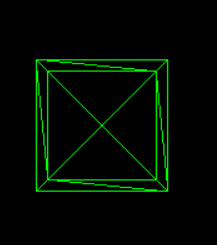
\includegraphics[width = \textwidth]{figs/ex_21_1.png}
        \caption{Cube visualized with perspective camera.}
        \label{fig:ex_21_1}
    \end{subfigure}%
    \begin{subfigure}{.5\textwidth}
        \centering
        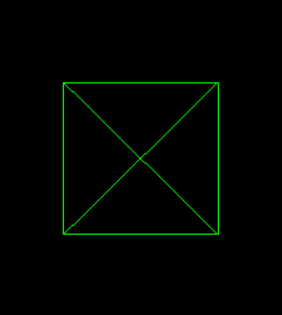
\includegraphics[width = \textwidth]{figs/ex_21_2.png}
        \caption{Cube visualized with orthographic camera.}
        \label{fig:ex_21_2}
    \end{subfigure}
\caption{Results of 2.1 - Camera models}
\label{fig:ex_21}
\end{figure}

As is it possible to notice, in Figure \ref{fig:ex_21_1} it is possible to see all the 6 squares that compose the cube, all six sides. On the other hand, in Figure \ref{fig:ex_21_2} only one square is possible to see.\par

This results are expected because perspective viewpoints simulates the way human eyes perceive the world by creating a sense of depth and distance. Objects that are farther away appear smaller than those that are closer. \newline
As for the orthographic viewpoints, objects are render without any sense of depth or distance meaning that all objects in the scene appear to be the same size, regardless of their distance from the camera.\par

As it is mention, it is necessary to respect the aspect ration of the camera. To assure that, calculations were done to compensate the width, maintaining/assuming the height constant; Figure \ref{figs:ex_21_code}.

\begin{figure}[!h]
    \centering
        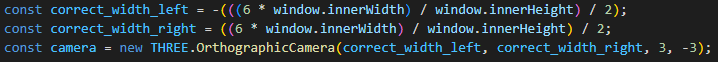
\includegraphics[width = \textwidth]{figs/ex_21_code.png}
        \caption{Code to apply the width correction and camera changing.}
        \label{figs:ex_21_code}
\end{figure}

%%%%%%%%%%%%%%%%%%%%%%%%%%%%%%%%%%%%%%%%%%%%%%%%%%%%%%%%%%
\section*{2.2 - Orbit control}
\label{ex_22}

In this exercise, students implement a three.js class that allow an easy control of the camera pose. To implement that, it is necessary to make an import of the class we pretended to use; we have tested the OrbitControls and TrackballControls. The controls are updated in the function that updates the view port.\par

Results are illustrated on Figure \ref{fig:ex_22}. The two images represent two different angles of view that the user desired to watch. The user clicked on the cube and dragged it chancing the angle.

\begin{figure}[!h]
\centering
    \begin{subfigure}{.5\textwidth}
        \centering
        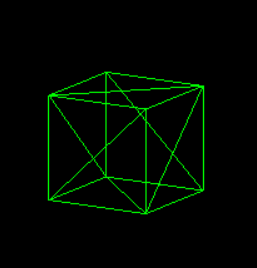
\includegraphics[width = \textwidth]{figs/ex_22_1.png}
        \caption{One angle.}
        \label{fig:ex_22_1}
    \end{subfigure}%
    \begin{subfigure}{.5\textwidth}
        \centering
        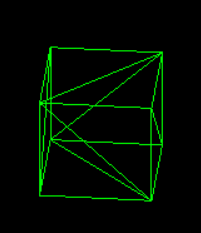
\includegraphics[width = \textwidth]{figs/ex_22_2.png}
        \caption{Other angle.}
        \label{fig:ex_22_2}
    \end{subfigure}
\caption{Results of 2.2 - Orbit control}
\label{fig:ex_22}
\end{figure}

%%%%%%%%%%%%%%%%%%%%%%%%%%%%%%%%%%%%%%%%%%%%%%%%%%%%%%%%%%
\section*{2.3 - Lighting and materials}
\label{ex_23}

In this exercise, lights are going to be added. Before that, we got back to the perspective camera, disabled the wireframe and turned the rotation of the cube back on.\par

We were asked to create create a DirectionalLight at position (0, 5, 0) with color 0xffffff, that is, white, and intensity equal to 1.0.\newline
In order for the object interact with the light, that is, light reflection is possible to see, it is needed a diferent material type from MeshBasicMaterial, in this case, a MeshPhongMaterial material. Finally, we added an ambient light.\par

In Figure \ref{fig:ex_23_1} it is represented the cube with only direction light; in Figure \ref{fig:ex_23_2} the cube with only ambient light; and finally, in Figure \ref{fig:ex_23_3}, the cube with both.

\begin{figure}[!h]
\centering
    \begin{subfigure}{.33\textwidth}
        \centering
        
\includegraphics[width = \textwidth]{figs/ex_23_1.png}
        \caption{Cube with only direction light.}
        \label{fig:ex_23_1}
    \end{subfigure}%
    \begin{subfigure}{.33\textwidth}
        \centering
        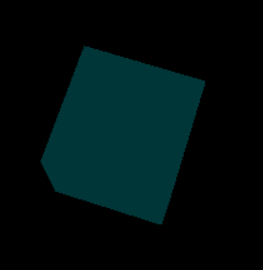
\includegraphics[width = \textwidth]{figs/ex_23_2.png}
        \caption{Cube with only ambient light.}
        \label{fig:ex_23_2}
    \end{subfigure}
    \begin{subfigure}{.33\textwidth}
        \centering
        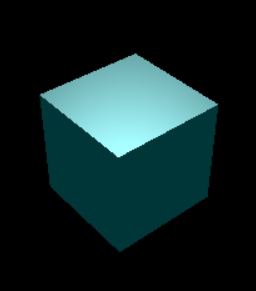
\includegraphics[width = \textwidth]{figs/ex_23_3.png}
        \caption{Cube with both lines}
        \label{fig:ex_23_3}
    \end{subfigure}
\caption{Results of 2.3 - Lighting and materials}
\label{fig:ex_23}
\end{figure}

In Figure \ref{fig:ex_23_1}, the direction light, we can see an ambient with its majority dark/off and a glimpse of the cube. In some angles it is possible to see a light reflection, which makes sense, because a direction light is pointing only in one direction, as the name says.\par

In Figure \ref{fig:ex_23_2} its only the ambient light and as it is possible to notice, the cube is seen 100\% and in a constant way which also makes sense.\par

Finally, combining the two lights, Figure \ref{fig:ex_23_3}, it is possible to always see the cube but, is some angles it is possible to see the reflection of the direction light.

%%%%%%%%%%%%%%%%%%%%%%%%%%%%%%%%%%%%%%%%%%%%%%%%%%%%%%%%%%
\section*{2.4 - Shading}
\label{ex_24}

In this exercise, students were asked to forget the cube and make two spheres.\newline
To the question "What do the widthSegments and heightSegments parameters correspond to?", this two parameters change the "form factor" of the sphere, that is, these parameters make the sphere smoother, with a more sphere-like shape, without seeing the segments that make them up.\newline
Then, we added ambient light and directional light from the previous exercise located between the two spheres with y=5.\newline
We were encouraged to modify the flatShading option of one of the materials by toggling between true and false and observe the result. The results are represented in Figure \ref{fig:ex_24}.

\begin{figure}[!h]
\centering
    \begin{subfigure}{.5\textwidth}
        \centering
        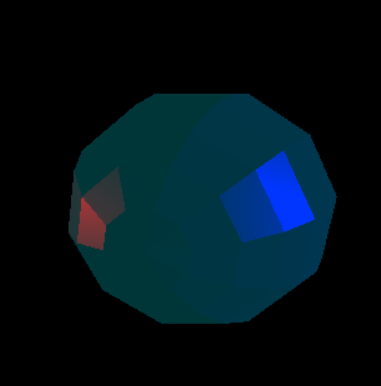
\includegraphics[width = \textwidth]{figs/ex_24_1.png}
        \caption{flatShading = true.}
        \label{fig:ex_24_1}
    \end{subfigure}%
    \begin{subfigure}{.5\textwidth}
        \centering
        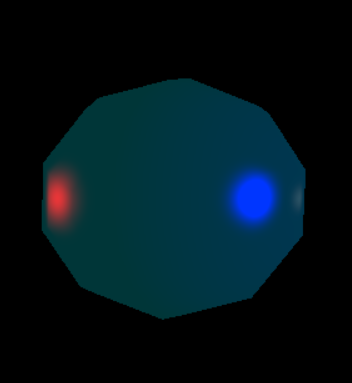
\includegraphics[width = \textwidth]{figs/ex_24_2.png}
        \caption{flatShading = false.}
        \label{fig:ex_24_2}
    \end{subfigure}
\caption{Results of 2.4 - Shading; flatShading}
\label{fig:ex_24}
\end{figure}

As it is possible to see, the difference is noticed when the light hits the sphere. When toggled true, the reflection is seen in the same shape of the segments that compose the object; when toggle false, it is sign as a "normal"/expected reflection.\par

As Optional/HomeWork, we applied MeshLambertMaterial type material to the spheres. This materials, the Lambertian, scatter light evenly in all directions so the specular coefficient and brightness are ignored. We also modify the properties of the spheres selecting values from a table to see the effects of different materials; we used emerald and gold.\newline
We also added a red directional light in position (-5,0,0) blue directional light in position (5,0,0) and a green spotlight light in position (0,0,-5) with angle Math.PI/20 and target object in (-2.5,0,0). The result obtained is represented in Figure \ref{figs:ex_24_3}.

\begin{figure}[!h]
    \centering
        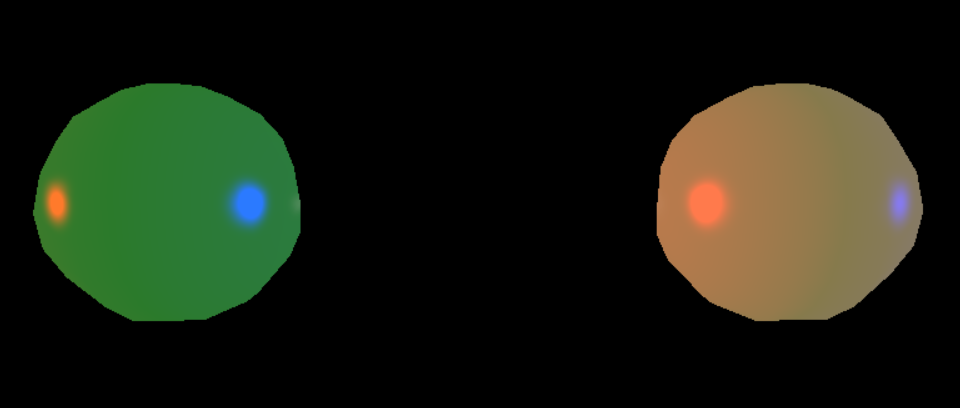
\includegraphics[width = \textwidth]{figs/ex_24_3.png}
        \caption{Results of 2.4 - Shading; Optional}
        \label{figs:ex_24_3}
\end{figure}

%%%%%%%%%%%%%%%%%%%%%%%%%%%%%%%%%%%%%%%%%%%%%%%%%%%%%%%%%%
\section*{2.5 - Transparency}
\label{ex_25}

Here, we added to the previews exercise two spheres with a slightly larger size around original spheres.\newline
We have used a glassed type material and played with the opacity and transparency parameters. The results can be found in Figure \ref{figs:ex_25}.

\begin{figure}[!h]
    \centering
        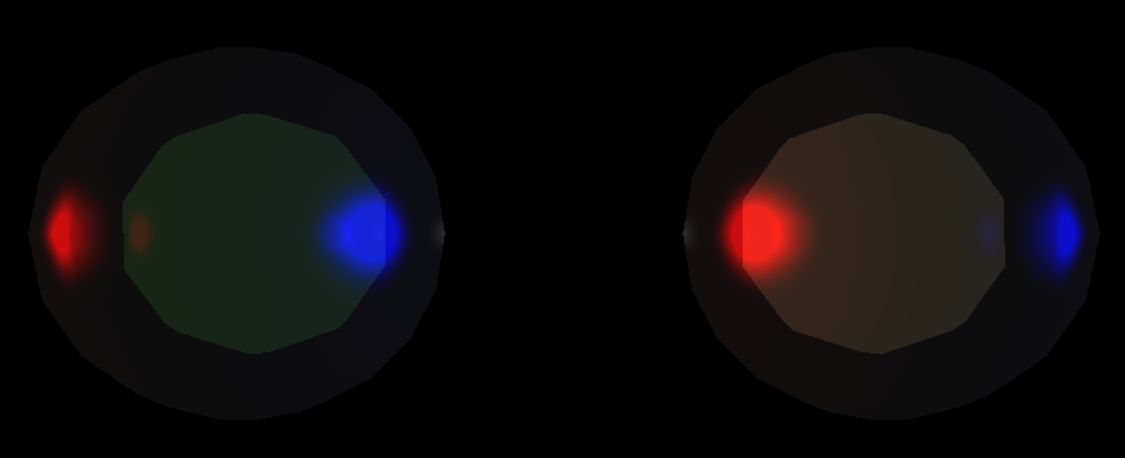
\includegraphics[width = \textwidth]{figs/ex_25.png}
        \caption{Results of 2.5 - Transparency}
        \label{figs:ex_25}
\end{figure}

As it is possible to notice, now the light reflection is hitting the transparent object but, a slight beam of light passes though the glass type material and hits the inner sphere. This made us concluded that this kind of material has realistic interactions with light because it reflects it, absorbs it and lets it through.

%%%%%%%%%%%%%%%%%%%%%%%%%%%%%%%%%%%%%%%%%%%%%%%%%%%%%%%%%%
\section*{2.6 - Transformations (scale and rotation)}
\label{ex_26}

In exercise 6, we have created a new scene that consisted of a box and four spheres as it is possible to see in Figure \ref{figs:ex_26}.

\begin{figure}[!h]
    \centering
        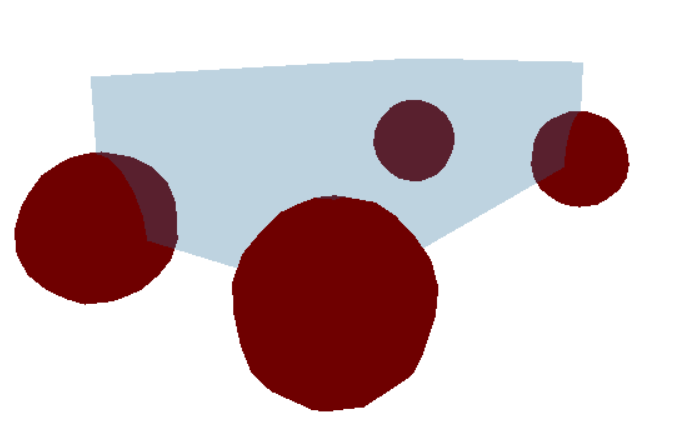
\includegraphics[width = \textwidth]{figs/ex_26.png}
        \caption{Results of 2.6 - Transformations (scale and rotation)}
        \label{figs:ex_26}
\end{figure}

We were informed that instead of adding multiple separate meshes, we could add multiple meshes into a single THREE.Object3D() via the add command - possible to see in the code developed \textbf{\href{https://github.com/goncalo-machado/VI}{here}}.

We were also asked to view the transformation matrices of the parallelipiped and of one of the spheres on the console. The transformation matrix is a 4 by 4 matrix used to store transformations done to an object and to perform further transformations.

\[
\begin{bmatrix}
a & b & c & \text{{tx}} \\
d & e & f & \text{{ty}} \\
g & h & i & \text{{tz}} \\
0 & 0 & 0 & 1
\end{bmatrix}
\]

In this matrix:
\begin{itemize}
    \item \( a, b, c \) represent the scaling and rotation components along the x, y, and z axes.
    \item \( d, e, f \) represent the scaling and rotation components along the x, y, and z axes.
    \item \( g, h, i \) represent the scaling and rotation components along the x, y, and z axes.
    \item \( \text{{tx}} \) represents the translation along the x-axis.
    \item \( \text{{ty}} \) represents the translation along the y-axis.
    \item \( \text{{tz}} \) represents the translation along the z-axis.
\end{itemize}

The top-left 3x3 matrix (\( \begin{bmatrix} a & b & c \\ d & e & f \\ g & h & i \end{bmatrix} \)) handles scaling and rotation, and the rightmost column (\( \begin{bmatrix} \text{{tx}} \\ \text{{ty}} \\ \text{{tz}} \end{bmatrix} \)) handles translation. The fourth row (0, 0, 0, 1) is a standard part of 4x4 matrices used in computer graphics.

This matrix is represented as an array of 16 elements with a column-major, meaning that the consecutive elements of a column are next to each other. For example, the element with index 0 is the \textit{a} variable in the example matrix, and the element with index 1 is the \textit{d} variable in the example matrix.

\begin{figure}[!h]
    \centering
        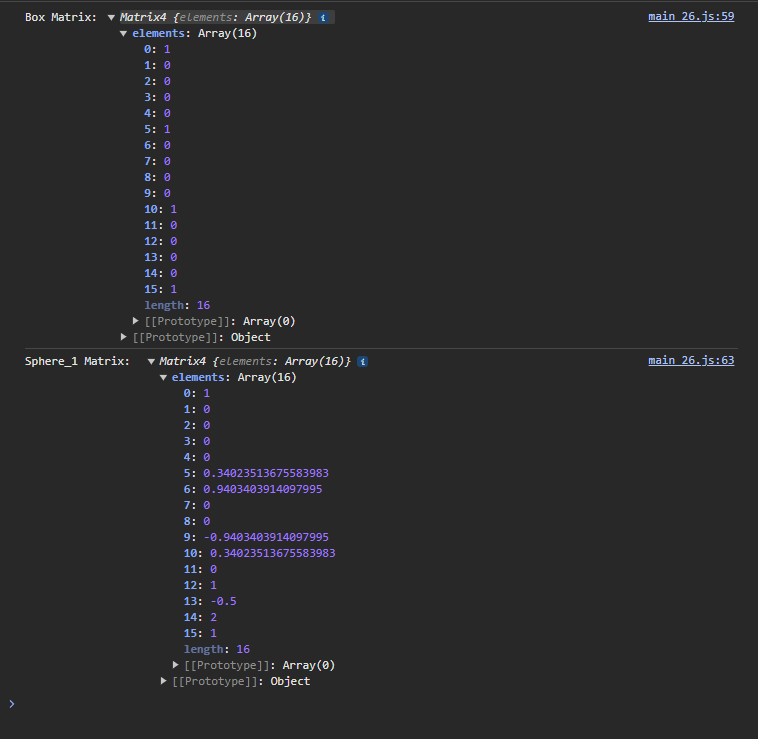
\includegraphics[width = \textwidth]{figs/ex_26_matrices.png}
        \caption{Transformation matrices of the parallelipiped ('Box') and of one of the spheres('Sphere\_1')}
        \label{figs:ex_26_matrices}
\end{figure}

As we can see from Fig \ref{figs:ex_26_matrices}, the parallelipiped has a very simple transformation matrix, since we place it with coordinates \(0,0,0\) and perform no transformation to it. The \textit{Sphere\_1} matrix is a little more complex, with some scaling and rotation components performed on the y and z axis due to the animation of the spheres. There is also a translation, which is represented in the elements with index 12,13 and 14, which correspond to the coordinates of the sphere.


%%%%%%%%%%%%%%%%%%%%%%%%%%%%%%%%%%%%%%%%%%%%%%%%%%%%%%%%%%
\section*{2.7 - Transformations (rotations)}
\label{ex_27}

For the finally exercise, we were asked to add to the previews exercise a new object that represents a coordinate system using three red, green, and blue cylinders (CylinderGeometry) for each axis.\newline
Another modification made was changing the spheres to cylinders.\newline
The result is represented in Figure \ref{figs:ex_27}.

\begin{figure}[!h]
    \centering
        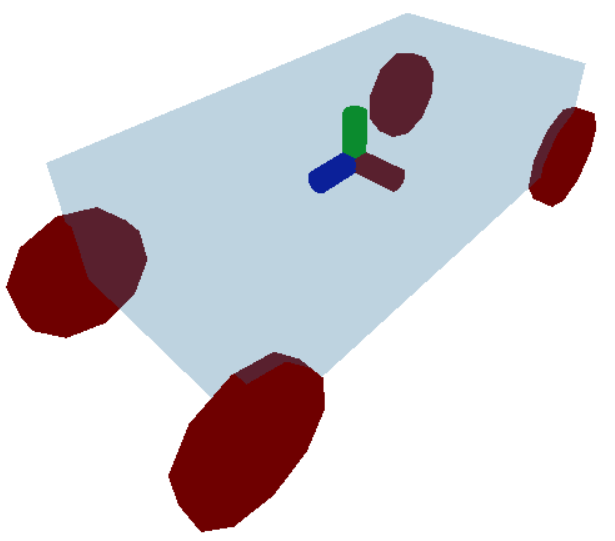
\includegraphics[width = \textwidth]{figs/ex_27.png}
        \caption{Results of 2.7 - Transformations (rotations)}
        \label{figs:ex_27}
\end{figure}

Note that an animation was requested. This consists in a moving car along a predefined circuit, in this case, a rotation of radius 1 around the point (0,0,-1)). Unfortunately, the animation is not possible to show but, once again, it is possible to see it \textbf{\href{https://github.com/goncalo-machado/VI}{here}}.\par

The axis cylinders were added to the box, like the spheres in Exercise \ref{ex_26} 2.6.\newline
It was necessary to rotate the cylinders that represent the wheels in $\pi$/2.\newline
For the three cylinders to represent a coordinate system, each of the cylinders needs the correct orientation. To the x axis, the cylinder was rotated $\pi$/2 in relation to the z; to the y axis, the cylinder was not rotated; and finally, the z axis, the cylinder was rotated $\pi$/2 in relation to the x.\par

To make the animation, we had to translate/update the box position (that include all the other objects, the axis and "wheels), which was achieved by using the following calculations:
\begin{lstlisting}

const radius = 1;
const angle = Date.now() * 0.001;

const translation_X = 0 + radius * Math.sin(angle);
const translation_Y = 0;
const translation_Z = -1 + radius * Math.cos(angle);

box.position.set(translation_X, translation_Y, translation_Z);

\end{lstlisting}

\noindent
The translation variables consist in the some of the point coordinates (0, 0, -1), then the sum of the radius of the rotation and, finally, the multiplication of the rotation angle. The Y axis remains constant throughout the animation. 

%%%%%%%%%%%%%%%%%%%%%%%%%%%%%%%%%%%%%%%%%%%%%%%%%%%%%%%%%%
\section*{Conclusion}
\label{Concl}

To sum up the Lesson 2 - Projections, lighting and transformations, focusing on camera models, lighting, shading, transparency, and transformations, was concluded with success as we explored differences between perspective and orthographic cameras, the effects of lighting on materials, and spatial manipulations completing successfully the exercises and presenting the expected results.

%%%%%%%%%%%%%%%%%%%%%%%%%%%%%%%%%%%%%%%%%%%%%%%%%%%%%%%%%%

\end{document}

